\appendix
\chapter{Installazione e Configurazione del lato Server}

    In questa sezione vediamo in maniera molto rapida come siamo riusciti a
    mettere in piedi il lato server per l'applicazione.


    \section{Apache CouchDB\texttrademark{}}

        Come prima cosa dobbiamo tenere a mente che Apache
        CouchDB\texttrademark{} non prevede la possibilità di gestire query
        spaziali e per questo motivo sarà necessario installare l'estensione
        Geocouch\footnote{Il repository GIT è reperibile all'indirizzo
        \url{https://github.com/couchbase/geocouch/tree/couchdb1.3.x}}.

        Nel nostro caso abbiamo installato tutto il lato server
        dell'applicazione su una macchina Arch Linux in quanto, per questo
        sistema, era presente tra i suoi repository software ufficiali la
        versione più aggiornata del DBMS (versione 1.5). Per installare Apache
        CouchDB\texttrademark{} è stato sufficiente il comando:
        \begin{lstlisting}[language=plane]
    sudo pacman -S couchdb
        \end{lstlisting}

        Una volta terminata l'installazione abbiamo reso
        il server raggiungibile dall'esterno modificando il file di
        configurazione \texttt{/etc/couchdb/default.ini}: all'interno della
        sezione \verb|[httpd]| abbiamo inserito l'indirizzo IP della macchina
        come mostrato nel segmento del file seguente.
        \begin{lstlisting}[language=plane]
[...]
    keyvalue_buffer_size = 2097152 ; value in bytes
    [httpd]
    port = 5984
    bind_address = 192.168.0.5
    authentication_handlers = {couch_httpd_oauth,oauth_authentication_handler},{couch_httpd_auth,cookie_authentication_handler},{couch_httpd_auth, default_authentication_handler}
[...]
        \end{lstlisting}
        A questo punto, una volta riavviato il servizio, il server è
        raggiungibile dall'esterno e può essere configurato comodamente dalla
        propria interfaccia web che in questo caso è raggiungibile dall'url
        \begin{lstlisting}[language=plane]
    http://192.168.0.5:5984/_utils/config.html
        \end{lstlisting}

        \noindent Adesso è necessario configurare:
        \begin{description}
            \item[cors] in modo che il server accetti messaggi \html{}
            particolari provenienti da un dominio differente da quello locale.
            In particolare, all'interno della sezione \texttt{cors}, bisogna
            settare i seguenti parametri:
            \begin{description}
                \item[credentials] va impostato a \texttt{true} in modo che il
                server controlli le credenziali di accesso allegate al
                messaggio HTTP che riceve;
                \item[headers] deve contenere l'elenco degli header HTTP che
                vogliamo siano accettati che nel nostro caso sono:
                \texttt{accept}, \texttt{authorization},\\
                \texttt{content-type}, \texttt{origin}, \texttt{x-titanium-id};
                \item[methods] devo contenere l'elenco dei metodi HTTP che
                vogliamo siano accettati e nel nostro caso sono: \texttt{HEAD},
                \texttt{GET}, \texttt{PUT}, \texttt{POST}, \texttt{DELETE};
                \item[origins] deve essere configurato in modo che vengano
                accettate richieste HTTP provenienti da qualsiasi dominio, per
                questo motivo abbiamo settato il valore ad \texttt{*}.
            \end{description}
            \item[couch\_httpd\_auth] in modo che vengano accettate solo richieste
            provenienti da utenti registrati; in particolare i parametri da
            configurare sono:
                \begin{description}
                    \item[require\_valid\_user] va impostato a \texttt{true}
                    proprio per il suddetto motivo;
                    \item[public\_fields] va impostato con un elenco dei campi
                    utente che vogliamo rendere pubblici; per la nostra
                    applicazione avevamo la necessità di avere i campi
                    \texttt{nick}, \texttt{mail} reperibili da qualsiasi altro utente;
                \end{description}
        \end{description}
        La configurazione completa è mostrata in fig. \ref{fig:confCouch1}.
        \begin{figure}[H]
            \centering
            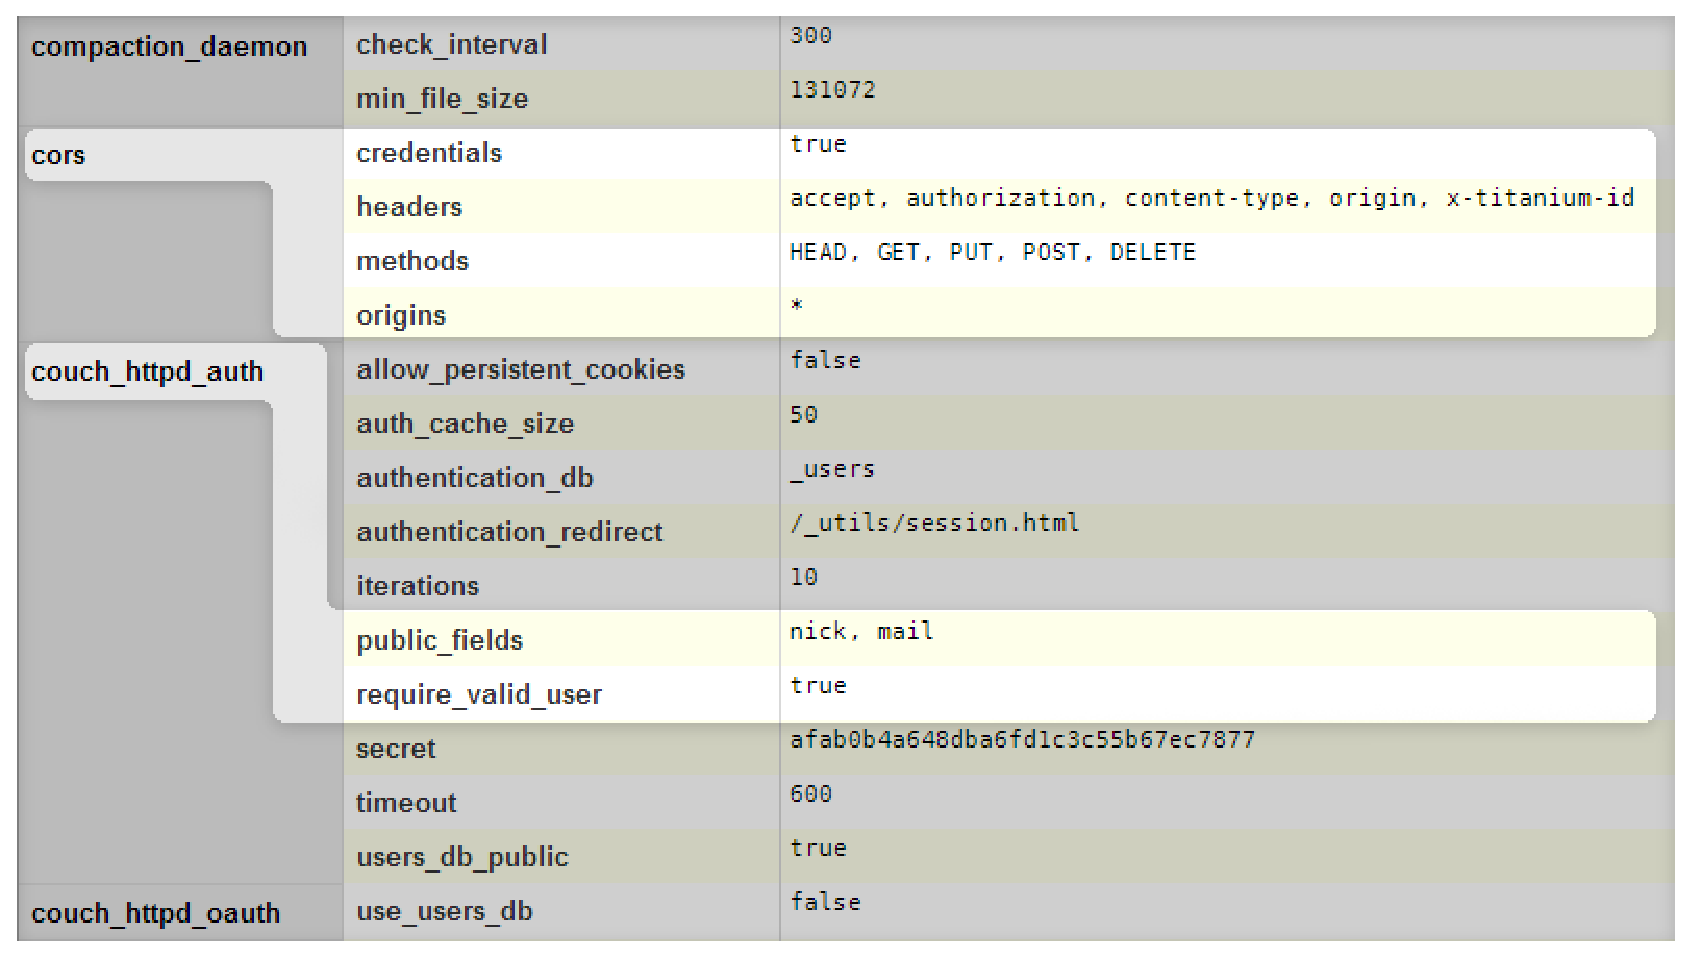
\includegraphics[keepaspectratio=true, width=0.99\textwidth]{couchConf1}
            \caption{
                Configurazione essenziale per rendere possibile la comunicazione
                della app con il server.
            }
            \label{fig:confCouch1}
        \end{figure}

        \subsection{Geocouch}
            Una volta che Apache CouchDB\texttrademark{} è stato installato e
            configurato abbiamo provveduto ad installare l'estensione per
            poter effettuare query spaziali sulle coordinate geografiche
            associate ad ogni segnalazione.

            Geocouch non è presente tra i repository standard di Arch Linux ma
            è disponibile in AUR (Arch User Repository)\footnote{Una guida
            completa su come utilizzare questo repository è disponibile
            all'url
            \url{https://wiki.archlinux.org/index.php/Arch_User_Repository_(Italiano)}.}
            così anche in questo caso siamo riusciti ad installare tutto con
            pochi semplici comandi:
            \begin{description}
                \item[ottenere il tarball]
                Prima di tutto è necessario recuperare il pacchetto
                contenente i sorgenti reperibile all'indirizzo
                \url{https://aur.archlinux.org/packages/ge/geocouch/geocouch.tar.gz}.
                \item[estrarre il pacchetto]
                Estrarre il tarball (preferibilmente in una cartella da tenere
                da parte solo per le compilazioni di AUR) con il comando
                \begin{lstlisting}[language=plane]
    tar -xzf geocouch.tar.gz
                \end{lstlisting}
                \item[compilare il pacchetto installabile]
                Lanciare il comando \texttt{makepkg} all'interno della directory
                contenente i file scaricati (il comando \texttt{makepkg -s} si
                occuperà di risolvere automaticamente le dipendenze tramite
                pacman). Questo scaricherà e compilerà il codice, infine
                creerà il pacchetto.
                \begin{lstlisting}[language=plane]
    cd geocouch/
    makepkg -s
                \end{lstlisting}
                \item[Intallare Geocouch]
                Installare il pacchetto ottenuto tramite \texttt{pacman}:
                \begin{lstlisting}[language=plane]
    sudo pacman -U geocouch-1.3.1-1-armv6h.pkg.tar.xz
                \end{lstlisting}
            \end{description}
            Terminata l'installazione è sufficiente un riavvio del servizio
            CouchDB per rendere operativa l'estensione installata.

        \subsection{Database e View}
            Vediamo ora come sono stati memorizzati i dati all'interno del
            DBMS, i DB utilizzati e quali view sono state definite per
            implementare le query a noi necessarie.

            \subsubsection{I dati memorizzati}
                Le entità che dovevano essere maneggiate sono state due: le
                segnalazioni e gli utenti. Andiamo a vedere come sono
                strutturate queste entità e in quali database sono collezionate

                \paragraph{Segnalazioni}
                Tutte le segnalazioni sono state memorizzate nel database di
                nome \texttt{degradi} ed ognuna di esse e composta dai seguenti
                campi:
                \begin{description}
                    \item[\_id] Un identificatore unico progressivo assegnato
                    dal server alla segnalazione una volta che questa viene
                    creata;
                    \item[\_rev] Un identificatore di revisione unico creato
                    dal server utilizzato per tenere traccia delle modifiche
                    fatte ad una certa segnalazione;
                    \item[\_attachments] Contiene l'immagine allegata alla
                    segnalazione. Per tutte le segnalazioni, la propria
                    immagine è nominata semplicemente \texttt{img};
                    \item[date] Contiene la data di creazione della
                    segnalazione espressa in millisecondi trascorsi da
                    EPOCH\footnote{Ore 00:00 del 1° gennaio 1970 (UTC);
                    maggiori dettagli a
                    \url{http://it.wikipedia.org/wiki/Tempo_(Unix)}.};
                    \item[loc] Contiene le coordinate geografiche della
                    posizione del degrado segnalato da questa segnalazione.
                    \texttt{loc} è composto da due valori:
                    \begin{description}
                        \item[latitude] La latitudine Nord espressa in gradi
                        decimali;
                        \item[longitude] La longitudine Est espressa in gradi
                        decimali.
                    \end{description}
                    \item[msg] Contiene una descrizione testuale del degrado
                    associato a questa segnalazione;
                    \item[title] Contiene un breve titolo per il degrado
                    associato a questa segnalazione;
                    \item[userId] Contiene l'identificatore unico dell'utente
                    che ha sottoposto questa segnalazione. Questo valore verrà
                    utilizzato per recuperare tutte le altre informazioni
                    dell'utente dal database degli utenti.
                \end{description}

                \paragraph{Utenti}
                Tutti gli utenti sono stati memorizzati nell'apposito DB di
                nome \texttt{\_users} già presente di default in Apache
                CouchDB\texttrademark{}. Ogni utente è composto da:
                \begin{description}
                    \item[\_id] Identificatore unico per un utente in Apache
                    CouchDB\texttrademark{} realizzato dall'applicazione al
                    momento della registrazione dell'utente stesso; è
                    realizzato concatenando la stringa
                    \texttt{org.couchdb.user:} con l'username scelto per
                    l'utente (nel nostro caso questo è lo UUID del dispositivo).
                    Il valore di \texttt{\_id} è quello inserito nel campo
                    \texttt{userId} nelle segnalazioni;
                    \item[\_rev] Un identificatore di revisione unico creato
                    dal server utilizzato per tenere traccia delle modifiche
                    fatte all'utente;
                    \item[derived\_key] Questo valore è creato dal server ed
                    è l'hash della concatenazione della password dell'utente e
                    del valore di salt;
                    \item[iteration] Questo valore è aggiunto dal server ed è
                    un parametro utilizzato nel calcolo dell'hash tra password
                    e salt;
                    \item[mail] Contiene l'indirizzo e-mail inserito
                    dell'utente al momento della sua registrazione; questo
                    valore come anche \texttt{nick} è pubblico e può essere
                    visualizzato anche da altri utenti;
                    \item[name] Username dell'utente registrato; nel nostro
                    caso corrisponde all'UUID del dispositivo che ha
                    registrato l'utente;
                    \item[nick] Nickname scelto dall'utente durante la fase di
                    registrazione; questo valore come anche \texttt{mail} è
                    pubblico e può essere visualizzato anche da altri utenti;
                    \item[password\_scheme] Valore scelto dal server e indica
                    il modo utilizzato dal server per calcolare l'hash tra
                    password e salt;
                    \item[roles] Vettore dei ruoli che l'utente ha nel
                    sistema. Questo campo è obbligatorio, ma non essendo a noi
                    necessario abbiamo specificato un vettore vuoto;
                    \item[salt] Questo valore è scelto a caso dal server e
                    viene utilizzato nel calcolo dell'hash della password;
                    \item[type] Specifica il tipo di utente che nel nostro
                    caso è un \texttt{user} e cioè un normalissimo utente.
                \end{description}
                Come password per un utente viene ancora utilizzato lo UUID
                del dispositivo che lo registra; questa, una volta fatta la
                registrazione, non compare mai nel database e viene
                memorizzata mediante i campi \texttt{derived\_key},
                \texttt{iterations}, \texttt{password\_scheme} e \texttt{salt}.

            \subsubsection{Le view}
                Per poter eseguire delle query è necessario prima definire
                delle view che sostanzialmente sono delle funzioni che
                implementano delle proiezioni sul specifici campi eseguite, in
                questo caso, su tutti gli utenti o su tutte le segnalazioni.
                Le definizioni di queste view sono memorizzate in appositi
                documenti all'interno dei DB sui quali queste view operano, in
                particolare: le view relative agli utenti sono memorizzate del
                documento \texttt{\_design/userQueries} all'interno del DB
                \texttt{\_users}, mentre quelle relative alle segnalazioni
                sono memorizzate nel documento \texttt{\_design/queries} del
                DB \texttt{degradi}.

                \paragraph{queries} Queste view sono quelle che operano sulle
                segnalazioni. Il documento le raccoglie in due gruppi diversi:
                \texttt{views} che sono le normali view e \texttt{spatial} che
                sono le query spaziali rese possibili da Geocouch.

                All'interno di \texttt{views} abbiamo:
                \begin{description}
                    \item[allDocsByUser] che restituisce record composti da i
                    campi \texttt{\_id}, \texttt{userId} e \texttt{title} di
                    tutte le segnalazioni ordinate per \texttt{userId};
                    \item[allDocsByDate] che restituisce tutte le segnalazioni
                    ordinate per il valore del loro campo \texttt{date}.
                \end{description}

                Per quanto riguarda le query spaziali, all'interno di
                \texttt{spatial} abbiamo:
                \begin{description}
                    \item[allDocsByLoc] che restituisce tutte le segnalazioni
                    ordinate sui valori di latitudine e longitudine.
                \end{description}

                La struttura completa dei questo documento è mostrata in
                figura \ref{fig:queries} mentre la sua definizione completa
                JSON è mostrata di seguito.
                \begin{lstlisting}[language=plane]
    {
      "_id": "_design/queries",
      "_rev": "13-a1bad8844225a755e1582d74493c5f8d",
      "spatial": {
        "allDocsByLoc": "function(doc) {
          if (doc.loc) {
            emit({
              type: \"Point\",
              coordinates: [doc.loc.longitude, doc.loc.latitude]
            },{
              userId: doc.userId,
              title: doc.title
            });
          }
        };"
      },
      "language": "javascript",
      "views": {
        "allDocsByUser": {
          "map": "function(doc) {
            emit(doc.userId, doc.title);
          }"
        },
        "allDocsByDate": {
          "map": "function(doc) {
            emit(doc.date, {
              _id: doc._id,
              userId: doc.userId,
              title: doc.title
            });
          }"
        }
      }
    }
                \end{lstlisting}
                \begin{figure}[H]
                    \centering
                    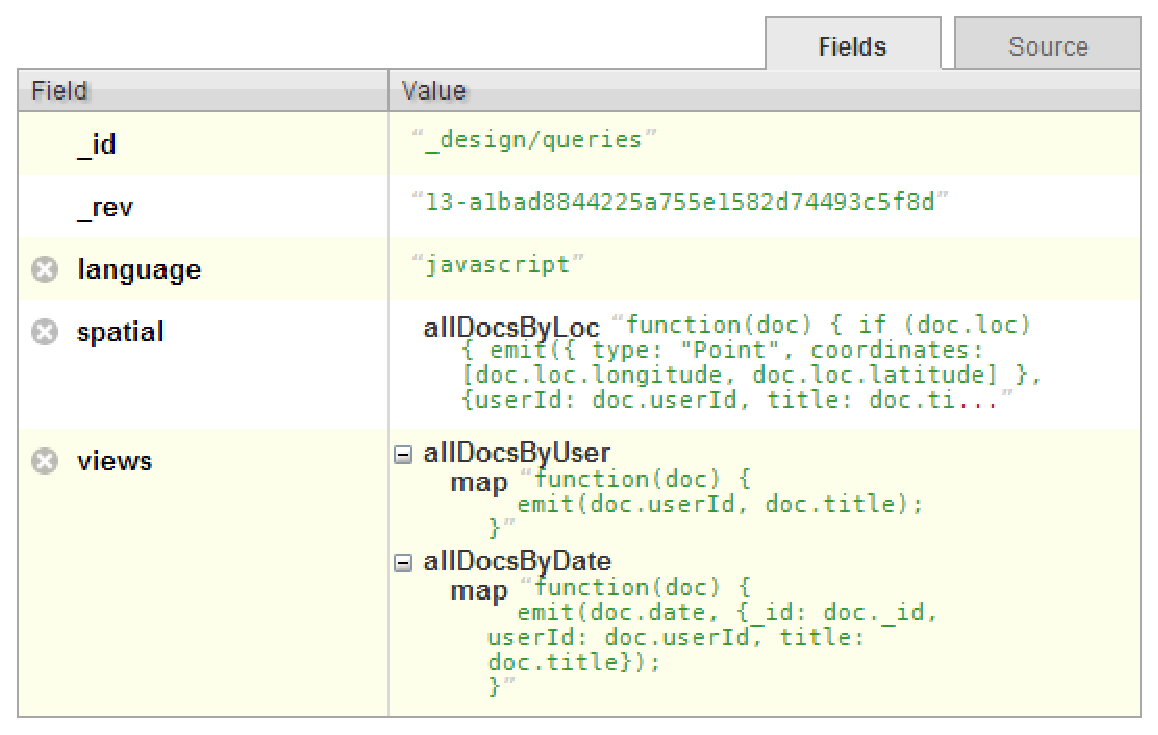
\includegraphics[keepaspectratio=true,
                    width=0.99\textwidth]{queries}
                    \caption{
                        Struttura del design document \texttt{queries} che
                        contiene le definizioni delle view applicabili alle
                        segnalazioni.
                    }
                    \label{fig:queries}
                \end{figure}
                Queste query possono sembrare poco utili ma, nei messaggi HTTP
                che vengono inviati al server per chiederne l'esecuzione,
                possono essere inseriti dei parametri per filtrare i risultati:
                in particolare è possibile ordinare tutte le segnalazioni per
                posizione e poi far restituire solo quelle presenti in una
                certa area. Per vedere quali parametri possono essere
                utilizzati nei messaggi HTTP di richiesta, fare riferimento
                alla documentazione di Apache CouchDB\texttrademark{}
                (\url{http://docs.couchdb.org/en/latest/api/ddoc/views.html}).

                \paragraph{userQueries} Queste view sono eseguibili sul
                database degli utenti. In questo caso è presente solo una sola
                view definita nel gruppo \texttt{views}:
                \begin{description}
                    \item[allNickandMail] Questa view ritorna tutti gli utenti
                    mostrando solo i loro campi pubblici, e cioè \texttt{nick}
                    e \texttt{mail}, ordinati per nickname.
                \end{description}
                La struttura completa di questo documento è mostrata in
                figura \ref{fig:userQueries} mentre la sua definizione completa
                JSON è mostrata di seguito.
                \begin{lstlisting}[language=plane]
    {
      "_id": "_design/usersQueries",
      "_rev": "2-d4c13f3a6e2b1f34c42c2a2224aef890",
      "language": "javascript",
      "views": {
        "allNickandMail": {
          "map": "function(doc) {
            emit(doc.nick, doc.mail);
          }"
        }
      }
    }
                \end{lstlisting}
                \begin{figure}[H]
                    \centering
                    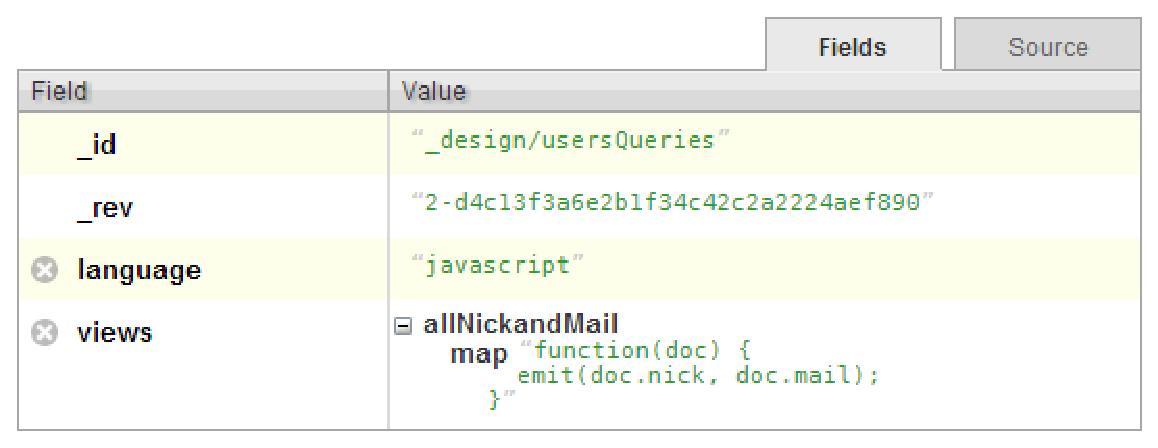
\includegraphics[keepaspectratio=true, width=0.99\textwidth]{userQueries}
                    \caption{
                        Struttura del design document \texttt{userQueries} che
                        contiene le definizioni delle view applicabili agli
                        utenti.
                    }
                    \label{fig:userQueries}
                \end{figure}


    \section{Node.js Web Server}
        Installare Node.js è stato immediato, anche questo software è
        presente nei repository ufficiali di Arch Linux quindi è sufficiente
        dare il comando
        \begin{lstlisting}
    sudo pacman -S nodejs
        \end{lstlisting}
        per avere a disposizione la versione 0.10.28-1. Una volta completata
        l'installazione si avranno a disposizione i comandi: \texttt{node}
        per avviare l'interprete o per eseguire un programma tramite file con
        codice sorgente, e \texttt{npm} che consente di installare nuovi
        moduli software per Node.js.

        Il codice del server consiste semplicemente di un unico file
        JavaScript di nome \texttt{degradoAmbientale.js}\footnote{Il file
        \texttt{degradoAmbientale.js} è disponibile al link:
        \url{https://github.com/pratesim/nodeServerDegradoAmbientale/blob/master/degradoAmbientale.js}}
        Questo server sfrutta i moduli \texttt{http} e \texttt{httpdispatcher}
        per accettare solamente richieste di registrazione provenienti
        dall'applicazione, e per comunicare all'applicazione
        stessa se l'utente è stato registrato correttamente oppure se esiste
        già un utente con il \texttt{nickname} presente nella richiesta di
        registrazione.

        Per poter utilizzare il server è quindi necessario installare i due
        suddetti moduli. Questo può essere fatto semplicemente tramite i comandi:
        \begin{lstlisting}[language=plane]
    sudo npm install -g http
    sudo npm install -g httpdispatcher
        \end{lstlisting}

        Inoltre bisogna personalizzare il codice del file
        \texttt{degradoAmbientale.js} con: le credenziali dell'amministratore
        del server CouchDB, con il numero della porta e l'ip della
        macchina sulla quale è presente il server CouchDB; e con il numero
        di porta e l'ip della macchina sulla quale si intende eseguire il
        server Node.js.
        In particolare vanno modificate le seguenti righe di codice
        \begin{lstlisting}[language=JavaScript]

    var admin = {
        name : '', //username admin server couchdb
        password : '' //password admin server couchdb
    };

    var options = {
        host:'192.168.0.111', //ip del server couchdb
        port: 5984, //porta del server couchdb
        auth: admin.name+':'+admin.password,
        path: '/_users',
        headers: {
            'Content-type':'application/json'
        },
        method: 'POST'
    };

    [...]

    //porta e ip della macchina contenente il server Node.js
    server.listen(1338, '192.168.0.103');
        \end{lstlisting}

        Infine per avviare il server è sufficiente eseguire il comando
        \begin{lstlisting}[language=plane]
    node degradoAmbientale.js
        \end{lstlisting}
